\newpage

\section{Simulation study}

\textbf{Section outline}
\begin{itemize}
    \item Motivate section. Explain the need for tuning the jump model. \textbf{Move description of estimator properties into Section 5.3 as it is not used before then.}
    \item Describe simulation procedure.
    \item Hyperparameter tuning. Important reader understands why we do this here and not on real data.
    \item Correct dists. Show boxplots. 
    \item Add plots of BAC's - \textbf{Missing}.
    \item Add Viterbi BAC as true BAC \textbf{Missing}
    \item Add additional boxplots with simulations sorted to all include 2 states.
    \item Mark best model estimates bold in \cref{tab:sim_misspec_t} and comment on this. \textbf{Missing}
    \item Make a plot of model performance when all data is sampled from one distribution only - to see how the estimators perform then on the longer sequences of data.
    \item Misspecified dists. Show boxplots. Consider adding plot of BAC's.
\end{itemize}

In this section HMMs are trained based on the estimation procedures described throughout \cref{section: estimation}. The primary purpose of the section is to compare how well different estimation methods converge toward the true parameter values when data is simulated from an HMM. Such analyses will not only provide valuable insights into the properties of the estimators, but also provide optimal values of certain hyperparameters used when using the models on real financial data. Of these hyperparameters, sample size is the most important one as it, in the following sections, is used in rolling models. In such a case, the trade-off in sample sizes is between faster adaptation of new information (shorter samples) and having a more consistent and robust estimator (longer samples). Additionally, the \jump estimator requires tuning of feature sets and jump penalty $\lambda$, which is this section covers. Before moving on with this analysis, some preliminary discussions on how to define classification accuracy and how to account for some inherent problems with HMMs is reviewed.

The advantage of using simulated data is that it entails knowing the true parameter values. Therefore, it becomes possible to directly analyze whether a model suggests parameter estimates close to the true values, as opposed to relying on general measures of fit such as AIC and BIC scores, which is necessarily the case when one works with real data. More importantly, simulated data allows for comparing the true state sequences with the estimated ones. This can be highly informative as it allows for measuring the accuracy in state classification. Simulations will be carried out under various alterations designed to test the models' convergence when some of their key assumptions about the data are (partially) unfulfilled\footnote
{Such as the maximum likelihood estimator, which assumes conditional normality. Since it has been shown that e.g. conditional students t-distributions are often a better fit the assumption is in practice often not fulfilled (Bulla et al. 2011).
}.

To test state classifications, accuracy of state predictions is defined using recall $\frac{tp}{tp+fn}$, where $tp$ is the number of true positives, and $fn$ is the number of false negative. It measures the percentage of actual positives that the model is able to detect correctly. When the true state is one, then the positive class will also be one, and the negative class will be all other predictions. When the true state is two the positive class will be two$,\ldots,$ and so on. However, one of the issues with recall is its inability to account for imbalanced data sets. To account for this, Nystrup et al. (2020) proposed using a balanced accuracy score (BAC), which is the average of accuracy in each observed state,
\begin{equation}
    BAC = \frac{1}{K} \sum_{k=1}^K \frac{tp_k}{tp_k + fn_k}
    \label{eq: BAC definition}
\end{equation}
where $tp_k$ is the number of true positives and $fn_k$ is the number of false negatives in state $k$. As a result, when a classifier performs equally well on all states, the BAC reduces to a regular accuracy, but if a classifier only performs well by always predicting the dominating class then BAC appropriately drops to the reciprocal of the number of states. Therefore, given data with two classes, if 99\% of the data belongs to the positive class and this is correctly detected, but the remaining 1\%, which belongs to the negative, is incorrectly classified, then the overall classifier obtains a BAC of 0.50, whereas regular accuracy would be 0.99. Considering the previously mentioned gain/loss asymmetry in financial returns where losses occur less frequently, yet their movements are larger than the corresponding movements in gains on average, BAC behaves as desired.

An inherent problem with comparing several HMMs is the fact that they output label-less states (predictions), which is due to their nature of being unsupervised machine learning models. This is not only the case in this simulation study, in which thousands of models are compared, but also when back-testing an HMM based on rolling windows on financial data. For example, consider training two HMMs by \mle on the same data with hidden states $a$ and $b$. The differences among the models' final parameter values and state sequences are then entirely attributable to the initialized parameter values (as explained in section \ref{section: estimation}, which are random quantities. If the models are initialized in a way where the first model labels state $a$ as 1 and state $b$ as 2 and the second model have the order reversed, it will make make a direct comparisons of the two perhaps equally good models difficult. There are several ways to circumvent this issue, such as choosing the labels that maximize the accuracy score, however, since this is not possible to do on real data where true states are unknown another method is used here. We rely on the fundamental assumption that the primary difference between conditional Gaussian states is the conditional variance $\sigma_k^2$, parameters and state labels are sorted according to variance. That is, we impose $\sigma_1^2 \leq \sigma_2^2$. Another option could have been sorting the states according to their means, however, when thinking about a "good" and "bad" state it is certainly a possibility to observe a state with a high mean and variance, which would still be interpreted as the "bad" state, thereby making such sorting a poor choice.


The rest of the section is structured as follows. Firstly, the simulation procedure is described. Secondly, a detailed analysis is conducted in order to tune the jump penalty $\lambda$ and feature set in the \jump model. Thirdly, once the penalty has been tuned, the models are trained on simulated data and compared. Initially, the models are trained on correctly specified conditional distributions. This is followed by an analysis that shows the models' performance when conditional distributions are purposely misspecified, since this is a realistic scenario when estimating HMMs on real data.

\subsection{Simulation procedure}

As described, data is simulated from a 2-state HMM throughout this section, yet in order to make the results comparable to those of Nystrup et al. (2020), the same parameters are chosen, thus yielding the Gaussian HMM.
\begin{equation*}
    O|\S \sim N(\mu_{st}, \sigma_{st}^2)
\end{equation*}
with parameters
$$
    \mu_{s_t}=
    \begin{cases}
        \mu_1= 0.0123 \\
        \mu_2= -0.0157
    \end{cases}, \quad
    \sigma_{s_t} =
    \begin{cases}
        \sigma_1 = 0.0347 \\
        \sigma_2 = 0.0778
    \end{cases}, \quad
    \mathbf{Q} = 
    \begin{bmatrix}
        0.9629 & 0.0371 \\
        0.2101 & 0.7899
    \end{bmatrix}
$$
The model is estimated by Hardy's (2001) using monthly returns, which has been shown to capture prominent stylized facts of financial times series such as volatility clustering and leptokurtosis well. There is a significant overlap between the two states, making it challenging to correctly infer the unobserved state sequence. By assuming instantaneous log returns follow a Lêvy process, the parameters are transformed from one time scale $t_1$ to another $t_2$ using
\begin{align*}
    \mu_s(t_1) / t_1 &= \mu_s(t_2) / t_2 \\
    \sigma_s(t_1) / \sqrt{\sigma_s(t_1)} &= \sigma_s(t_2) / \sqrt{\sigma_s(t_2)} \\
    Q(t_1)^{1/t_1} &= Q(t_2)^{1/t_2}
\end{align*}

where $\mu(t), \sigma(t)$ and $Q(t)$ are parameters associated with time scale $t$. Assuming there is twenty trading days in a month, i.e. $t_{monthly}=20$ and $t_{daily}=1$, monthly parameters are transformed into daily
$$
    \mu_{s_t}=
    \begin{cases}
        \mu_1= 0.0615 \times 10^{-2} \\
        \mu_2= -0.0785 \times 10^{-2}
    \end{cases}, \quad
    \sigma_{s_t} =
    \begin{cases}
        \sigma_1 = 0.7759 \times 10^{-2} \\
        \sigma_2 = 1.7400 \times 10^{-2}
    \end{cases}, \quad
    Q = 
    \begin{bmatrix}
        0.9979 & 0.0021 \\
        0.0120 & 0.9880
    \end{bmatrix}
$$

Each series simulated from this model is generated as follows. Firstly, the element $s_0$ is drawn from the stationary distribution $\pi$, and each subsequent element is drawn from $q_{t-1}$, i.e. the row of $Q$ corresponding to the last state sojourn. Based on the value of each $s_t$, observations $o_t$ are generated from the conditional distributions. By repeating this procedure, 1000 different series are simulated with sample lengths $H = 250, 500, 1000, 2000$

\subsection{Hyperparameter tuning in \jump model}
\label{subsection: jump_penalizer}
Since the \mle model does not contain any hyperparameters (except for sample size in a rolling model), it can be applied to the simulated data directly. However, this is not the case for the \jump model which requires a given value for the jump penalty $\lambda$ as well as the generation of times series features. As previously mentioned, the objective is to test the models' ability to correctly identify state sequences, hence the best \jump model is the one to maximize BAC with respect to $\lambda$. Since BAC is a random quantity\footnote
{It is a function of the data and the initial state sequence $s_0$, which in the \jump estimator is generated by K-means++. Both quantities are random.},
it is appropriate to define the estimator $\Omega(\lambda)= E[BAC|\lambda]$, which is maximized with respect to $\lambda$. This can be defined as, 
\begin{equation}
    \hat\Omega(\lambda) = \frac{1}{N} \sum_{i=1}^N BAC_{i, \lambda}^H
\end{equation}
where $N$ is the amount of simulated series, and $BAC_{i, \lambda}^H$ refer to the BAC of the $i$th sequence of sample size $H$ computed using a \jump model with penalty $\lambda$.

Having defined these properties the analysis proceed by computing $BAC_{i, \lambda}^H$ on sample lengths $H =$ 250, 500, 1000 and 2000. Furthermore, the jump penalties are considered on a grid defined on the logarithmic scale with base 2. Initially the grid was defined on a logarithmic scale with base 10, but evidently this was too broad to yield meaningful results. As such, the grid points are equidistantly placed on the closed interval logarithmic scale $[2^{-2}, 2^{7}]$. This operation is repeated for a number of feature sets explained next.


\subsubsection{Selecting the optimal jump penalizer and feature set}
\label{subsubsection: optimal jump penalizer}
One of the main challenges when it comes to selecting the jump penalizer is to determine which features to show the model during estimation. This type of analysis is desirable to conduct since it makes it possible to compare performance across different feature sets, at a very low computational expense. For instance, if a feature's impact on BAC is minimal, it might reduce the model's overall ability of obtaining significant results, since the feature will be clustered with noise and randomness whereas other features might severely improve BAC. As such, selecting the features for estimation of the jump penalizer is includes an inherent bias-variance trade-off.  

We proceed by training three different feature sets on the simulated data and subsequently computing their average BAC scores $\hat\Omega(\lambda)$ for each simulation length H. Many more feature sets were tried, but with similar or worse results than reported here. The reader should note that the analysis will not conclude whether the selected feature space is optimal since there is currently no method of doing so. This is because an unlimited amount of features can be derived from the log return series (Tansjö, 2020). 

Using windows length of $l = 6$ and $l = 14$, the first feature set is defined as in algorithm \ref{algo:jump_features_set_1}. 

\begin{algorithm}[H]
\KwInput{Time series O, and window length $l$}
\BlankLine
1. Observation: $o_t$\;
2. Left absolute change: $|o_t-o_{t-1}|$ \;
3. Previous left absolute change: $|o_{t-1}-o_{t-2}|$ \;
4. Left local mean: $mean(o_{t-l},\ldots,o_{t})$ \;
5. Left local std: $std(o_{t-l},\ldots, o_{t})$ \;
6. Left local median: $median(o_{t-l},\ldots,o_{t})$ \;
\BlankLine

\KwOutput{Feature set 1, where each each feature $z_i$ is standardized as $z_i = \frac{\bar x-x_i}{\sigma}$}
\caption{Feature set 1 used in \jump estimation of HMM's}
\label{algo:jump_features_set_1}
\end{algorithm}

The results from the simulation, based on the features from algorithm \ref{algo:jump_features_set_1}, are shown in figure \ref{fig: BAC plot feature set 1}. It is evident by the figure that there is a substantial difference between the sample lengths and their respective BAC. Overall the BAC is increasing in sample length as long as the jump penalizer is below $2^4$ (except for $H=250$).

\begin{figure}[H] 
    \centering
    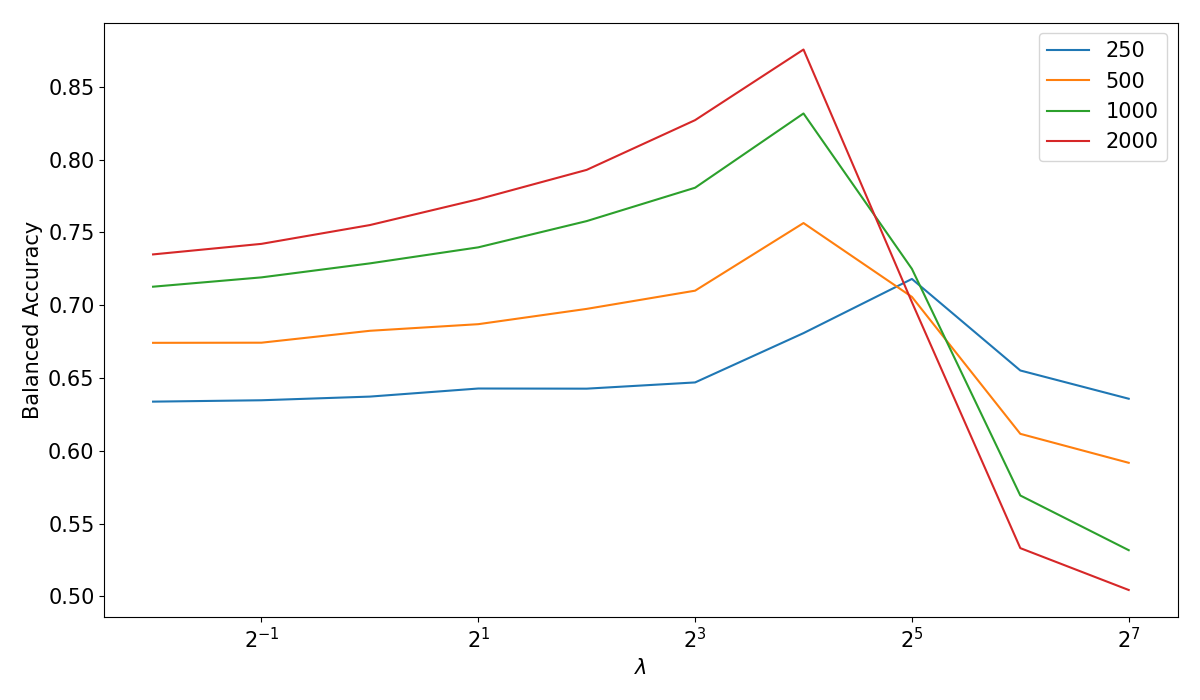
\includegraphics[width=1\textwidth]{analysis/model_convergence/images/jump_penalties_feature_set_1.png}
    \caption[Balanced accuracy of \jump estimator using feature set 1]{Balanced accuracy of \jump estimator as a function of the penalty $\lambda$ using different simulation lengths and the features defined in algorithm \ref{algo:jump_features_set_1}. All points in the plot are based on the estimate $\hat{\Omega} (\lambda)$ which includes 1000 simulated series for each sample length.}
    \label{fig: BAC plot feature set 1}
\end{figure}

An interesting point is the varying sensitivity of the jump penalizer $\lambda$ across the different sample lengths. As such, it is evident from figure \ref{fig: BAC plot feature set 1} that the optimal BAC is achieved for different levels of $\lambda$ across sample lengths. For sample lengths of 250 the BAC is maximized when $\lambda = 2^5$, however, for sample lengths 500, 1000 and 2000 the BAC is maximized when $\lambda = 2^4$. An explanation for this behaviour might be explained by the fact that the probability of only having one state is increasing when sample size decreases\footnote
{Since sampled states are implicitly geometrically distributed.
}
and thus increasing $\lambda$ also decrease the amount of state switches. Another explanation is that the feature set simply is insufficient for \jump models, because, as we will see next other feature sets doesn't have differences in optimal values of $\lambda$.

As mentioned in \cref{subsection: Jump theory}, when $\lambda$ grows large enough, which for the features defined in algorithm \ref{algo:jump_features_set_1} is when $\lambda > 2^4$, the \jump estimator only identifies the dominating state, hence the BAC drops towards 0.50. This is a natural consequence of its definition in equation \ref{eq: BAC definition}. Following this, when $\lambda$ is sufficiently small, BAC converges to the unpenalized case, which is essentially the same as applying a K-means model where the time ordering of observations becomes irrelevant. 

The results showcased by figure \ref{fig: BAC plot feature set 1} indicate that the jump penalizer should be chosen as $\lambda = 2^4$ since this is around the level in which the BAC is maximized for sample lengths 500, 1000 and 2000. However, the steep curvature of BAC indicates that the optimal value is quite unstable for this feature set, and thus a slightly wrong value of $lambda$ on either side of the optimum, will result in steep decline in model performance. As a consequence of this a new feature set will be defined and tested. The feature set will entail a variety of different parameters that are typically found in technical analysis trading strategies. The window length remains identical to that of feature set 1.

\begin{algorithm}[H]
\KwInput{Time series O, and window length $l$}
\BlankLine
1. Min/Max difference: $max(o_{t-l},\ldots,o_{t}) - min(o_{t-l},\ldots,o_{t})$ \;
2. Exponential moving average (EMA) 10 days: $a * o_t + (1-a) * EMA_{t-1}$, \quad where $a$ is the smoothing factor, $a = \frac{2}{10+1}$ \;
3. Upper Bollinger band: $mean(o_{t-l},\ldots,o_t) + 1.96 * std(o_{t-l},\ldots,o_t)$ \;
4. Lower Bollinger band: $mean(o_{t-l},\ldots,o_t) - 1.96 * std(o_{t-l},\ldots,o_t)$\;
5. Bollinger band width: $Upper\ Bollinger\ Band - Lower\  Bollinger\ Band$ \;
6. Bollinger band \%B: $\frac{mean(o_{t-l},\ldots,o_{t}) - Lower\ Bollinger\ band} {Upper\ Bollinger\ band - Lower\ Bollinger\ band}$  \;
\BlankLine
\KwOutput{Feature set 2, where each each feature $z_i$ is standardized as $z_i = \frac{\bar x-x_i}{\sigma}$}
\caption{Feature set 2 used in \jump estimation of HMM's}
\label{algo:jump_features_set_2}
\end{algorithm}

The results based on the features from algorithm \ref{algo:jump_features_set_2} are shown in figure \ref{fig: BAC plot feature set 2}. It is evident from the figure that BAC again is generally increasing in the sample length. This is in line with the results obtained through feature set 1.

\begin{figure}[H] 
    \centering
    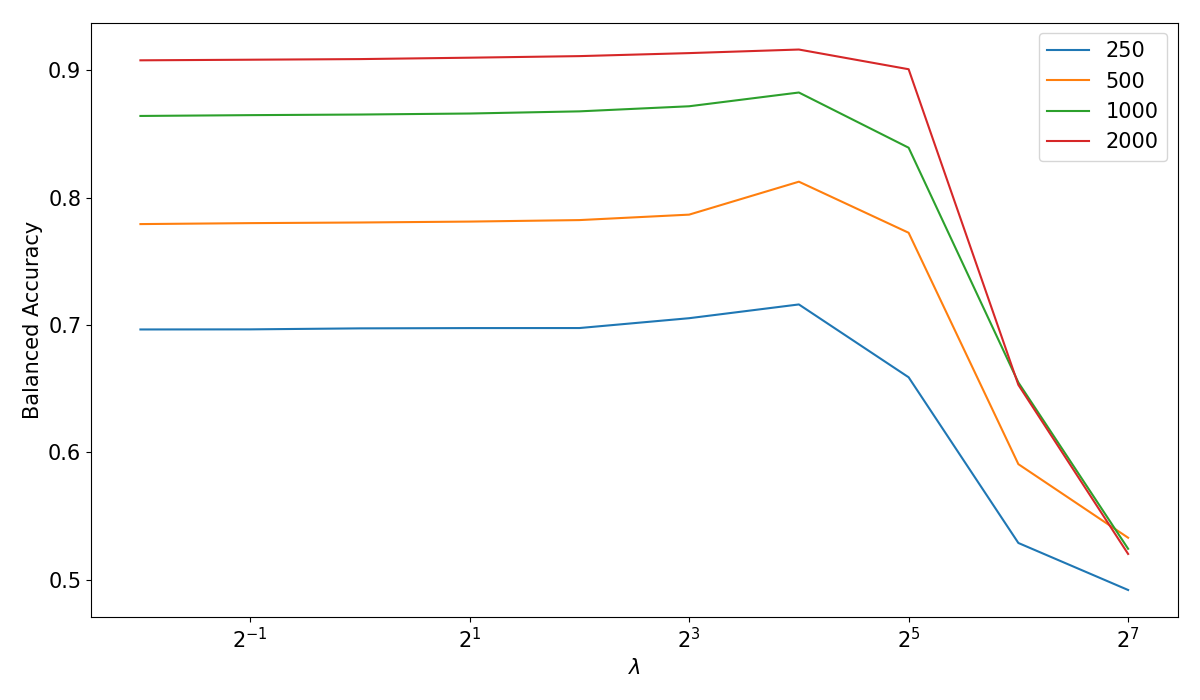
\includegraphics[width=1\textwidth]{analysis/model_convergence/images/jump_penalties_feature_set_2.png}
    \caption[Balanced accuracy of \jump estimator using feature set 2]{Balanced accuracy of \jump estimator as a function of the penalty $\lambda$ using different simulation lengths and the features defined in algorithm \ref{algo:jump_features_set_2}. All points are based on the estimate $\hat{\Omega} (\lambda)$ based on 1000 simulated series.}
    \label{fig: BAC plot feature set 2}
\end{figure}

Interestingly, it appears that the BAC is less sensitive to changing jump penalizers compared to figure \ref{fig: BAC plot feature set 1}. This is evident since the BAC is a horizontal line, for all sample lengths, when the jump penalizer lies in the range $2^{-2}$ to $2^3$. The horizontal line is a favourable property as it provides a higher confidence in the selected size of the jump penalizer since state prediction results will be consistent across $\lambda$. Furthermore, it is evident that the the BAC have been shifted upwards, for all sample lengths, when compared to the results from figure \ref{fig: BAC plot feature set 1}. This means that the features defined in algorithm \ref{algo:jump_features_set_2} appear to be much stronger in achieving accurate state predictions. 

Finally, it was evident by figure \ref{fig: BAC plot feature set 1} that the different sample lengths appeared to maximize BAC for different levels of $\lambda$, however, when analysing figure \ref{fig: BAC plot feature set 2} it appears that the BAC maximizes at the same $\lambda$ for all sample lengths. This property further provides confidence when selecting the optimal level of $\lambda$, since the result is unanimous across sample lengths. As such, the results showcased by figure \ref{fig: BAC plot feature set 2} indicate that the jump penalizer should be chosen as $\lambda = 2^4$ since this is where BAC is maximized for all sample lengths. This finding is particularly interesting because this is the same size of $\lambda$ that was suggested by using the features defined in feature set 1. Therefore, the conclusion from both feature sets point towards a jump penalizer of the size $2^4$, although the second feature set achieves a much higher BAC across samples and jump penalizers. Due to these findings an appropriate analysis would be to make an identical analysis which include all features as defined in algorithm \ref{algo:jump_features_set_3}. The corresponding grid plot is shown in figure \ref{fig: BAC plot feature set 3}.

\begin{algorithm}[H]
\KwInput{Time series O, and window length $l$}
\BlankLine
1. Observation: $o_t$\;
2. Left absolute change: $|o_t-o_{t-1}|$ \;
3. Previous left absolute change: $|o_{t-1}-o_{t-2}|$ \;
4. Left local mean: $mean(o_{t-l},\ldots,o_{t})$ \;
5. Left local std: $std(o_{t-l},\ldots, o_{t})$ \;
6. Left local median: $median(o_{t-l},\ldots,o_{t})$ \;
7. Min/Max difference: $max(o_{t-l},\ldots,o_{t}) - min(o_{t-l},\ldots,o_{t})$ \;
8. Exponential moving average (EMA) 10 days: $a * o_t + (1-a) * EMA_{t-1}$, \quad where $a$ is the smoothing factor, $a = \frac{2}{10+1}$ \;
9. Upper Bollinger band: $mean(o_{t-l},\ldots,o_t) + 1.96 * std(o_{t-l},\ldots,o_t)$ \;
10. Lower Bollinger band: $mean(o_{t-l},\ldots,o_t) - 1.96 * std(o_{t-l},\ldots,o_t)$\;
11. Bollinger band width: $Upper\ Bollinger\ Band - Lower\  Bollinger\ Band$ \;
12. Bollinger band \%B: $\frac{mean(o_{t-l},\ldots,o_{t}) - Lower\ Bollinger\ band} {Upper\ Bollinger\ band - Lower\ Bollinger\ band}$  \;
\BlankLine
\KwOutput{Feature set 3, where each each feature $z_i$ is standardized as $z_i = \frac{\bar x-x_i}{\sigma}$}
\caption{Feature set 3 used in \jump estimation of HMM's}
\label{algo:jump_features_set_3}
\end{algorithm}


\begin{figure}[H] 
    \centering
    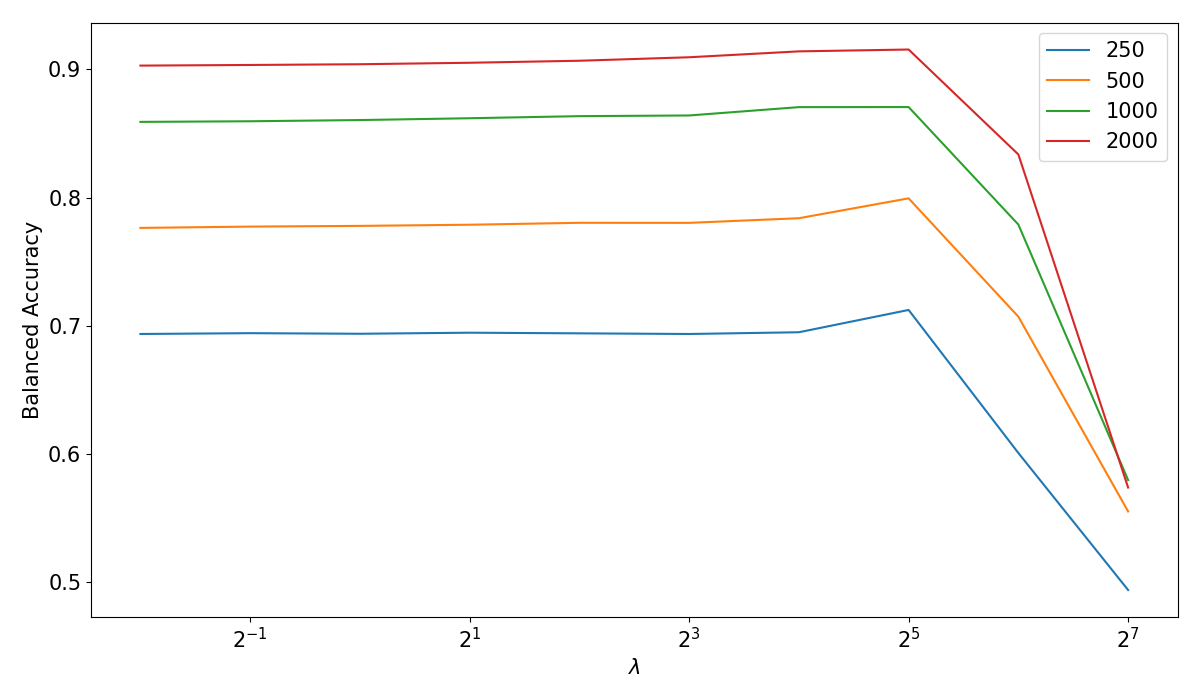
\includegraphics[width=1\textwidth]{analysis/model_convergence/images/jump_penalties_feature_set_3_all.png}
    \caption [Balanced accuracy of \jump estimator using feature set 3]{Balanced accuracy of \jump estimator as a function of the penalty $\lambda$ using different simulation lengths and the features defined in algorithm \ref{algo:jump_features_set_3}. All points are based on the estimate $\hat{\Omega} (\lambda)$ based on 1000 simulated series.}
    \label{fig: BAC plot feature set 3}
\end{figure}

Evidently, several interesting aspects occur when using all the defined features from algorithm \ref{algo:jump_features_set_3} to determine the jump penalizer. Firstly, the plots of the BAC against the jump penalizers becomes stable for a larger domain of definition, since the plots are horizontal for jump penalizers in the range of $2^{-2}$ to $2^5$, which is longer compared to that of figure \ref{fig: BAC plot feature set 2}. Secondly, the BAC is shifted slightly upwards in figure \ref{fig: BAC plot feature set 3} compared to figure \ref{fig: BAC plot feature set 2}. This means that using all the features result in a slightly better BAC compared to solely relying on the features defined in algorithm \ref{algo:jump_features_set_2}. Furthermore, a particular interesting finding is the apparent shift of the optimal jump penalizer. As such, it is evident from figure \ref{fig: BAC plot feature set 3} that the BAC maximizes when $\lambda$ is $2^5$, for all sample lengths. This is contrary to the findings from figure \ref{fig: BAC plot feature set 1} and \ref{fig: BAC plot feature set 2} both pointing towards an optimal jump penalizer of $2^4$ though it is unsurprising since the optimal jump penalty is increasing in number of dimensions of the feature set. Despite this inconsistency, all 3 feature sets point towards a jump penalizer in the range of $2^4$ to $2^5$, which contribute to a high confidence when selecting the $\lambda$.

In addition, it can be concluded from the analysis of the 3 feature sets, that increasing the sample length increases the BAC. As such, further analysis should consider testing longer sample lengths across different feature sets in order to uncover an optimal combination that pushes  the BAC even higher. This is because it appears that there is a fast decreasing marginal increase in BAC of using additional features, evident by comparing figure \ref{fig: BAC plot feature set 2} and \ref{fig: BAC plot feature set 3}. Conclusively, due to the fact that the BAC is slightly larger and horizontal for a longer domain of definition, for all sample lengths, the jump penalizer will be selected based on the feature set defined in algorithm \ref{algo:jump_features_set_3}. However, rather than using the optimum value of $\lambda=2^5$ we will proceed with $\lambda=2^4$ due to the fact that BAC is steeply decreasing for too high values of $\lambda$ but rather flat if $\lambda$ is lower than the optimum.

\subsection{Simulation study with correctly specified distributions}
\label{section:simulation_corspeciffied}
As this simulation section is largely concerned with the comparison of estimators, it is appropriate to outline some general desirable properties that estimators should fulfill. Three general properties of estimators are unbiasedness, consistency and efficiency. Unbiasedness refers to whether expected value of the estimator equals the true value, i.e $E(\hat\theta)=\theta$. This section will primarily focus on consistency, which refer to an estimator $\hat\theta$ converging in probability to $\theta$ as a function of sample size $n$. Denoting $\hat\theta_n$ as an estimator trained on $n$ samples, the property is fulfilled if, in the limit, the following holds
\begin{align}
    \lim_{n\to\infty} E(\hat\theta) &= \theta \\
    \lim_{n\to\infty} Var(\hat\theta) &= 0
\label{eq:sim_consistency}
\end{align}

Thus, as the sample size increases one generally wants to see that the estimates converge towards the true values while the distribution simultaneously shrinks around the true values. A neat way of investigating whether this property holds, for both the \mle and \jump estimator, is by using boxplots as shown further below. Finally, the efficiency of the estimators $\hat\theta_{mle}$, $\hat\theta_{jump}$ is compared by checking their variances, with the most efficient being the one with the narrowest distribution.

\cref{tab:jump_gaussian} and \cref{fig:jump_normal_box} summarizes the performance of the \mle and \jump estimator for various sample sizes when compared to the true values. As mentioned, data is generated from a two-state gaussian HMM. Apart from the model parameters, estimated BAC is reported for each model. Accuracy for for the true parameters are obtained by running the Viterbi algorithm using an HMM with the true model parameters. This can be seen as a measure of best obtainable performance in state detection and is used to get a sense of where the 'upper bound' on BAC lies when comparing the other models.

\textbf{Add Viterbi results for true BAC}
\begin{table}[H]
\centering
\caption[Estimates from conditional Gaussian distributions of the \mle and \jump parameters and their convergence towards the true values]{Estimates of the \mle and \jump parameters and their convergence towards the true values as a function of simulation length. Results are based on 1000 simulations from conditional Gaussian distributions.}
\begin{tabular}{llrrrrrr}
\toprule
     &      &  $\mu_1$ &  $\mu_2$ &  $\sigma_1$ &  $\sigma_2$ &  $q_{11}$ &  $q_{22}$ \\
sample_size & model &          &          &             &             &           &           \\
\midrule
250  & true &   0.0006 &  -0.0008 &      0.0078 &      0.0174 &    0.9979 &    0.9880 \\
     & mle &   0.0017 &  -0.0000 &      0.0052 &      0.0121 &    0.7410 &    0.9658 \\
     & jump &   0.0006 &  -0.0001 &      0.0079 &      0.0113 &    0.9770 &    0.8903 \\
500  & true &   0.0006 &  -0.0008 &      0.0078 &      0.0174 &    0.9979 &    0.9880 \\
     & mle &   0.0015 &  -0.0002 &      0.0060 &      0.0139 &    0.8152 &    0.9719 \\
     & jump &   0.0006 &  -0.0003 &      0.0079 &      0.0130 &    0.9834 &    0.8898 \\
1000 & true &   0.0006 &  -0.0008 &      0.0078 &      0.0174 &    0.9979 &    0.9880 \\
     & mle &   0.0011 &  -0.0006 &      0.0071 &      0.0160 &    0.9208 &    0.9763 \\
     & jump &   0.0006 &  -0.0006 &      0.0080 &      0.0152 &    0.9866 &    0.9420 \\
2000 & true &   0.0006 &  -0.0008 &      0.0078 &      0.0174 &    0.9979 &    0.9880 \\
     & mle &   0.0008 &  -0.0007 &      0.0076 &      0.0171 &    0.9823 &    0.9817 \\
     & jump &   0.0006 &  -0.0007 &      0.0080 &      0.0164 &    0.9951 &    0.9679 \\
\bottomrule
\end{tabular}

\label{tab:jump_gaussian}
\end{table}

\begin{figure}[H] 
    \centering
    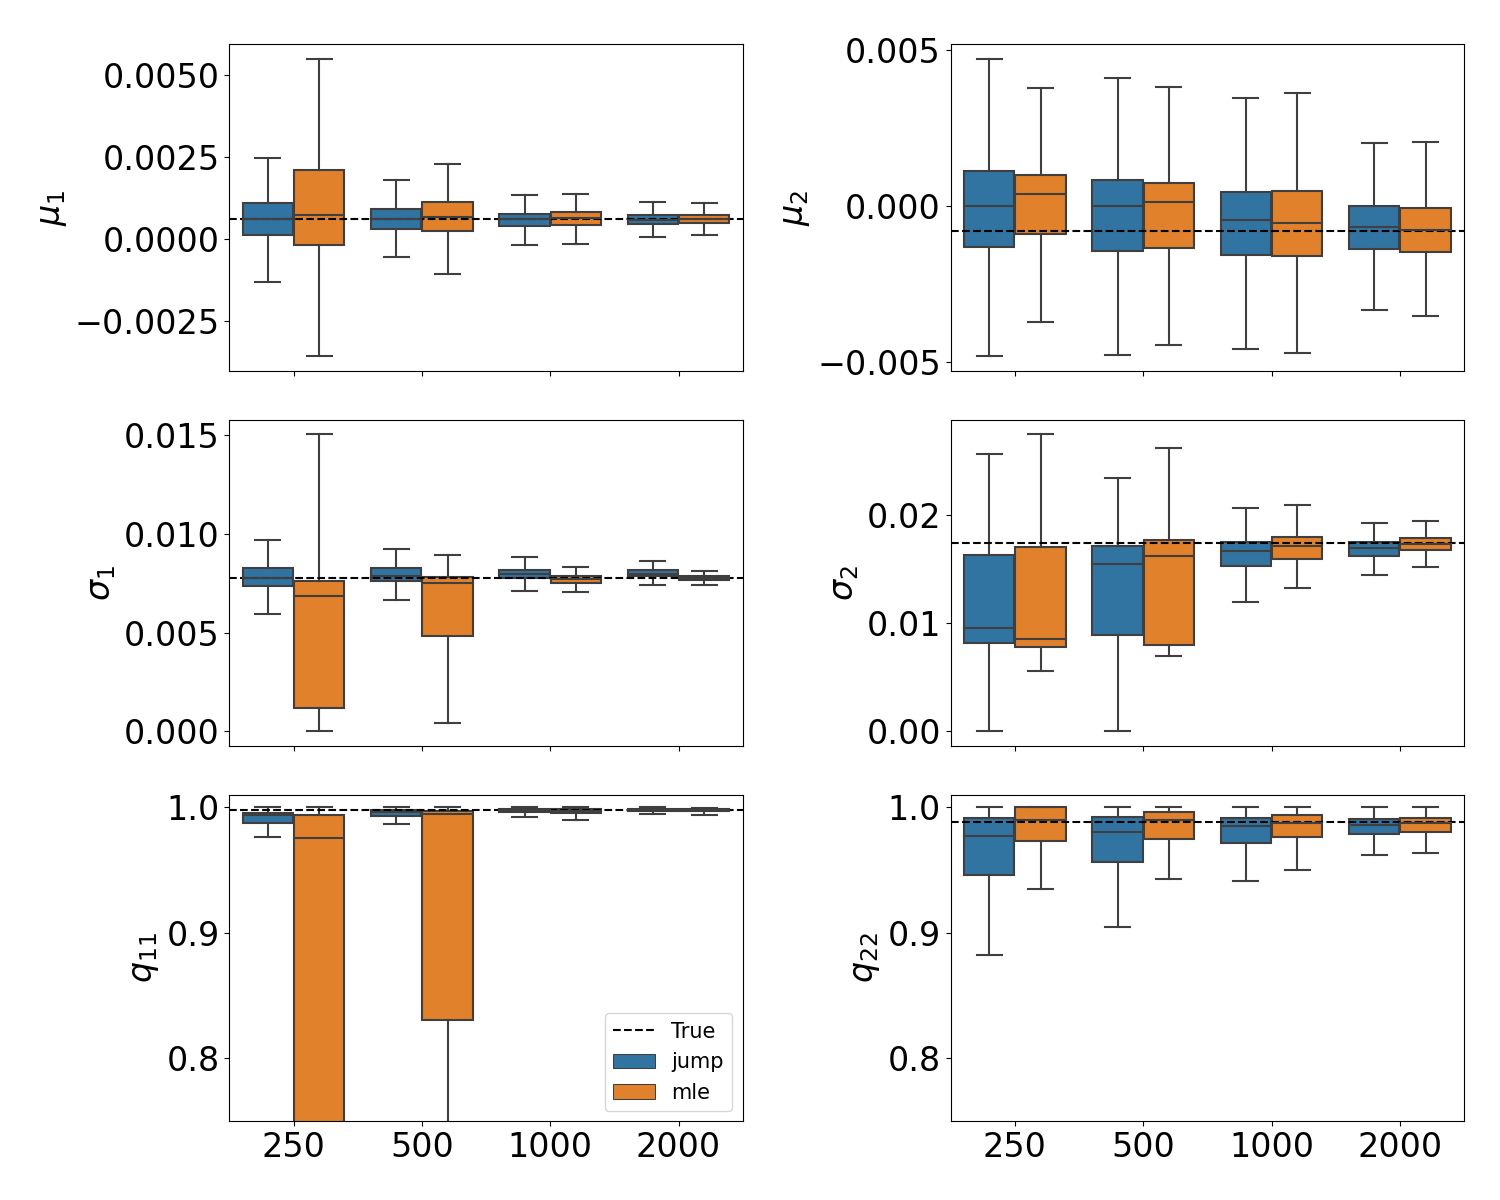
\includegraphics[width=1\textwidth]{analysis/model_convergence/images/simulation_normal_box.png}
    \caption[Boxplot of \mle and \jump parameter estimates from correctly specified conditional Gaussian distributions]{Boxplot of the \mle and \jump parameter estimates from correctly specified Gaussian distributions. The estimates show the models' convergence towards the true parameter values as a function of simulation length. Results are based on 1000 simulations.}
    \label{fig:jump_normal_box}
\end{figure}

\textbf{Add boxplot of BAC for both estimators separately about here.}

It is clear that both models converge towards the true values as a function of simulation length. Both estimators appear to fulfill the consistency property outlined in \cref{eq:sim_consistency} for all model parameters since their distributions becomes more narrow around the true values when sample size increases. Curiously, the \jump estimator is able to detect the low-variance state quite accurately, even at the shortest simulation lengths as evident by its narrow distribution in $q_{11}$.

Still, both models performs poorly on the high-variance state for simulation lengths below 1000 as evident by their medians for $\sigma_2$ being quite far from the true value. This is most likely explained by the fact that, at short simulation lengths the probability of seeing both states are quite low. For a series of 250 observations the probability of only seeing one state is 51\%, at 500 observations it is 30\%, for 1000 observations it is 10\% and at 2000 observations it is 1\%\footnote
{These probability are calculated using the fact that sojourn times follows a geometric distrubution, as $\sum_{i=1}^K q_{ii}^H\pi_i$, where H is the sample length and $i$ denotes the state.
}. 
When only one state is observed, it becomes inherently harder for the estimator to detect that only one state is actually present, when it is designed to fit two. This is most clearly evident from the \mle model's estimate of $q_{11}$, which for sample size 250 and 500 is very inconsistent, but at length 1000 and above becomes very consistent about the true value.

\cref{fig:jump_normal_box} show the same results, but with those simulation sequences only containing one state removed. It is clear that both estimators become much more consistent for all estimates, as the distributions are narrower and converges faster than before. Most notably, the \mle model is now fitting $q_{11}$ much better than in \cref{fig:jump_normal_box}. Previous studies such as Zheng et al. (2019), has alleviated the problem by excluding those simulations with only one state present as shown in \cref{fig:jump_normal_box}. However, this introduces bias in the transition probabilities. The problem with excluding those simulations, is that when training HMMs on real data, then it possible that only one state will be present at times. This is especially true when one is considering a rolling window. In such cases, it is important that the estimator doesn't break down, which seems to be the case for the \mle estimator at shorter sample sizes. On samples of 1000 observations and above, both models do comparatively well though convergence speed quickly decreases for sequences longer than 2000.

\begin{figure}[H] 
    \centering
    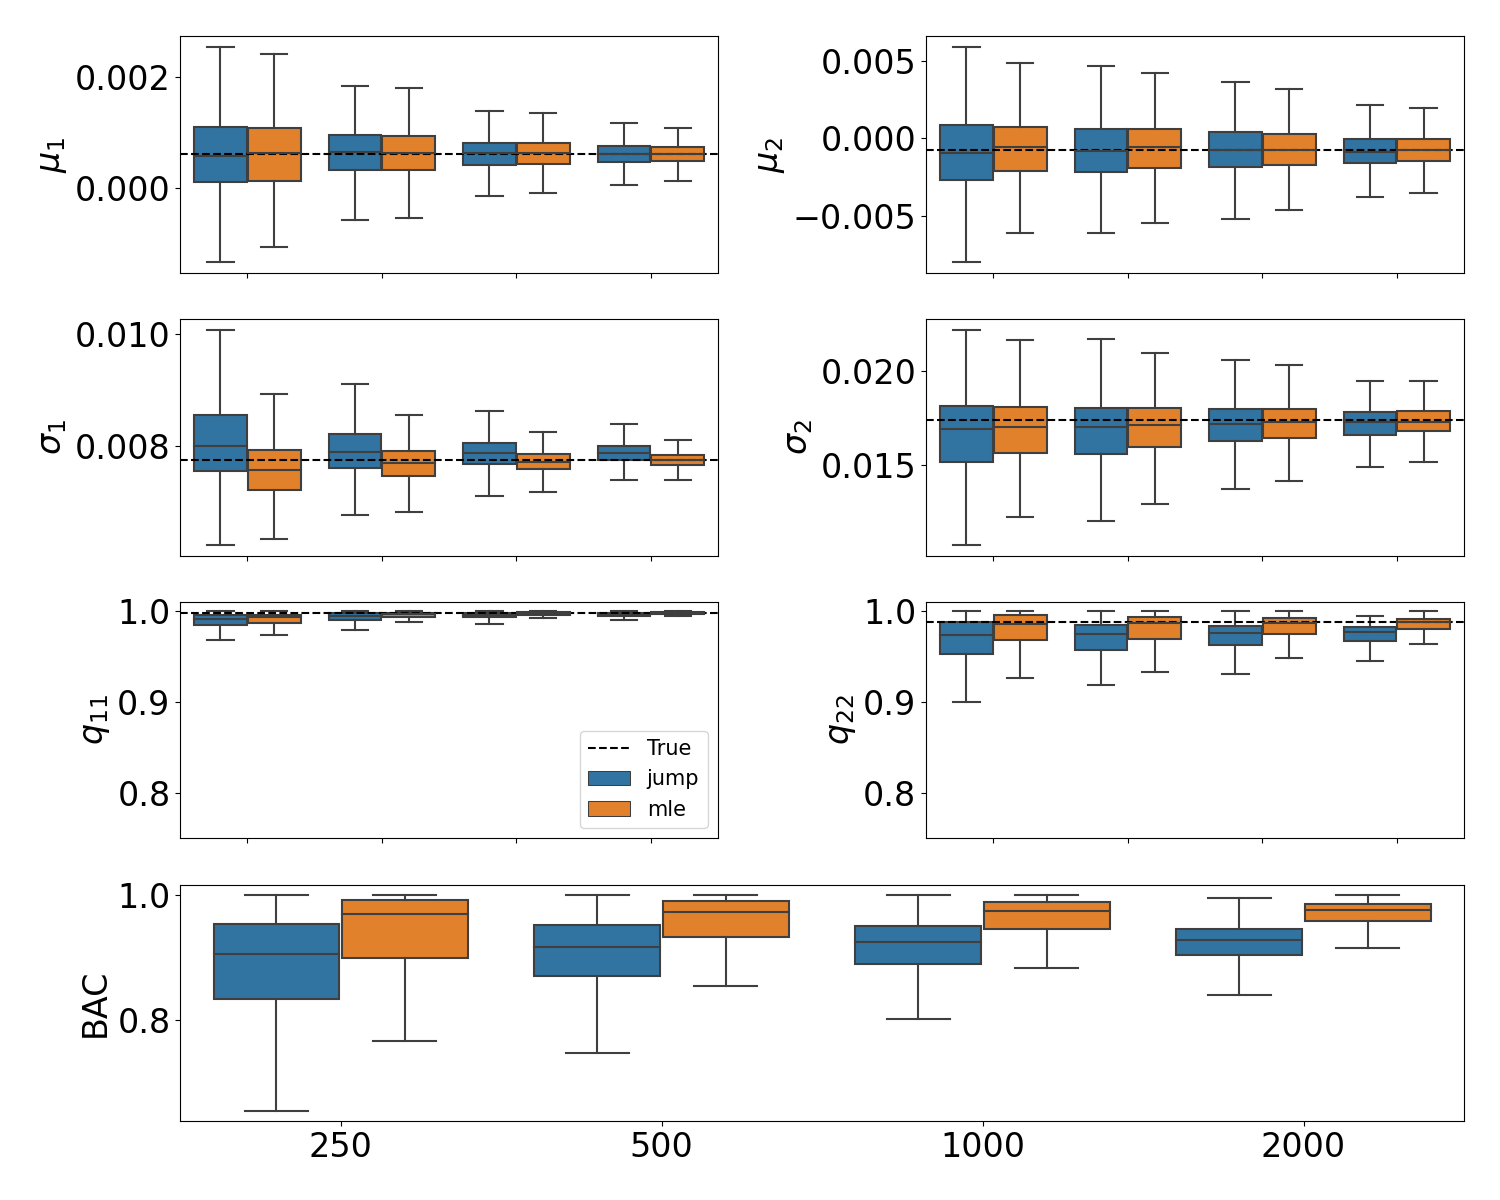
\includegraphics[width=1\textwidth]{analysis/model_convergence/images/simulation_normal_box_2states.png}
    
    \caption [Boxplot of \mle and \jump parameter estimates from correctly specified conditional Gaussian distributions with five degrees of freedom. Sorted version] {Boxplot of the \mle and \jump parameter estimates from correctly specified Gaussian distributions with five degrees of freedom. The estimates show the models' convergence towards the true parameter values as a function of simulation length. Results are based on 1000 simulations which are sorted to only include those where both states are present. \textbf{Consider moving to appendix.}}
    \label{fig:jump_normal_box_2states}
\end{figure}

In conclusion, the different estimators generally converge towards the true parameter values when the simulation length is increased. However, these results are dependent on the assumption that the underlying distribution of data is known, which is generally unrealistic - especially with financial returns. In the following section we show how the estimators perform when they are purposefully estimated on an unknown distribution, which is not a mixture of gaussian distributions.


\subsection{Simulation study with misspecified distributions}
\label{section:simulation_misspecified}

In this section, the simulation procedure from before is repeated, except for the fact that observations are sampled from conditional student's t distribution instead of gaussian, though means, variances and transition probabilities remain unchanged. The simulated t-distribution has five degrees of freedom. Student's t distribution generally have fatter tails, and have been shown to better resemble financial returns compared to normal distributions (Cont, 2001). As such, the goal of this section is to create a more realistic simulation experiment, in which models are still specified to be conditional gaussian, even though the simulated data is not. When implementing these types of models in a portfolio, it is important to know how it performs in such an environment. The results in this section will thus provide insights into how well each estimator performs in such a scenario, and where they fail. A preliminary check in \cref{fig:jump_theoretical_fit} confirms that, provided the models can correctly identify the states, then they should be able to estimate the true values quite accurately even though both models are gaussian HMMs.

\cref{fig:jump_t_box} shows the mean parameter values as a function of simulation length based on 1000 simulations. Compared to \cref{fig:jump_normal_box}, both estimators performance has generally worsened as evident by the transition probabilities. Yet, the \jump estimator is generally more robust, especially when analyzing the transition probabilities, in which the \jump estimator has close to similar performance as before. As mentioned in \cref{subsection: Jump theory}, a large advantage of the \jump model is that, during training it does not assume anything about the distributional properties of the data, therefore making it more robust when the data's distribution is unknown.

\begin{table}[H]
\centering

\caption[Estimates from conditional t-distributions of the \mle and \jump parameters and their convergence towards the true values]{Estimates of the \mle and \jump parameters and their convergence towards the true values as a function of simulation length. Results are based on 1000 simulations from conditional t-distributions with five degrees of freedoms.}
\begin{tabular}{llrrrrrr}
\toprule
     &      &   $\mu_1$ &   $\mu_2$ &  $\sigma_1$ &  $\sigma_2$ &    $q_11$ &    $q_22$ \\
sample_size & model &           &           &             &             &           &           \\
\midrule
250  & true &  0.000615 & -0.000785 &    0.007759 &    0.017397 &  0.997900 &  0.988000 \\
     & mle &  0.002475 &  0.002068 &    0.012354 &    0.012383 &  0.700296 &  0.733797 \\
     & jump &  0.000591 &  0.000125 &    0.009567 &    0.017927 &  0.980719 &  0.942377 \\
500  & true &  0.000615 & -0.000785 &    0.007759 &    0.017397 &  0.997900 &  0.988000 \\
     & mle &  0.001878 &  0.002102 &    0.013870 &    0.014039 &  0.757573 &  0.737563 \\
     & jump &  0.000640 & -0.000103 &    0.009677 &    0.019699 &  0.985360 &  0.945942 \\
1000 & true &  0.000615 & -0.000785 &    0.007759 &    0.017397 &  0.997900 &  0.988000 \\
     & mle &  0.001769 &  0.002351 &    0.014671 &    0.014961 &  0.797976 &  0.789653 \\
     & jump &  0.000648 & -0.000627 &    0.009694 &    0.021009 &  0.988130 &  0.946477 \\
2000 & true &  0.000615 & -0.000785 &    0.007759 &    0.017397 &  0.997900 &  0.988000 \\
     & mle &  0.001107 &  0.001388 &    0.015695 &    0.015464 &  0.850219 &  0.857551 \\
     & jump &  0.000657 & -0.000836 &    0.009689 &    0.021683 &  0.990051 &  0.941516 \\
\bottomrule
\end{tabular}

\label{tab:sim_misspec_t}
\end{table}

\begin{figure}[H] 
    \centering
    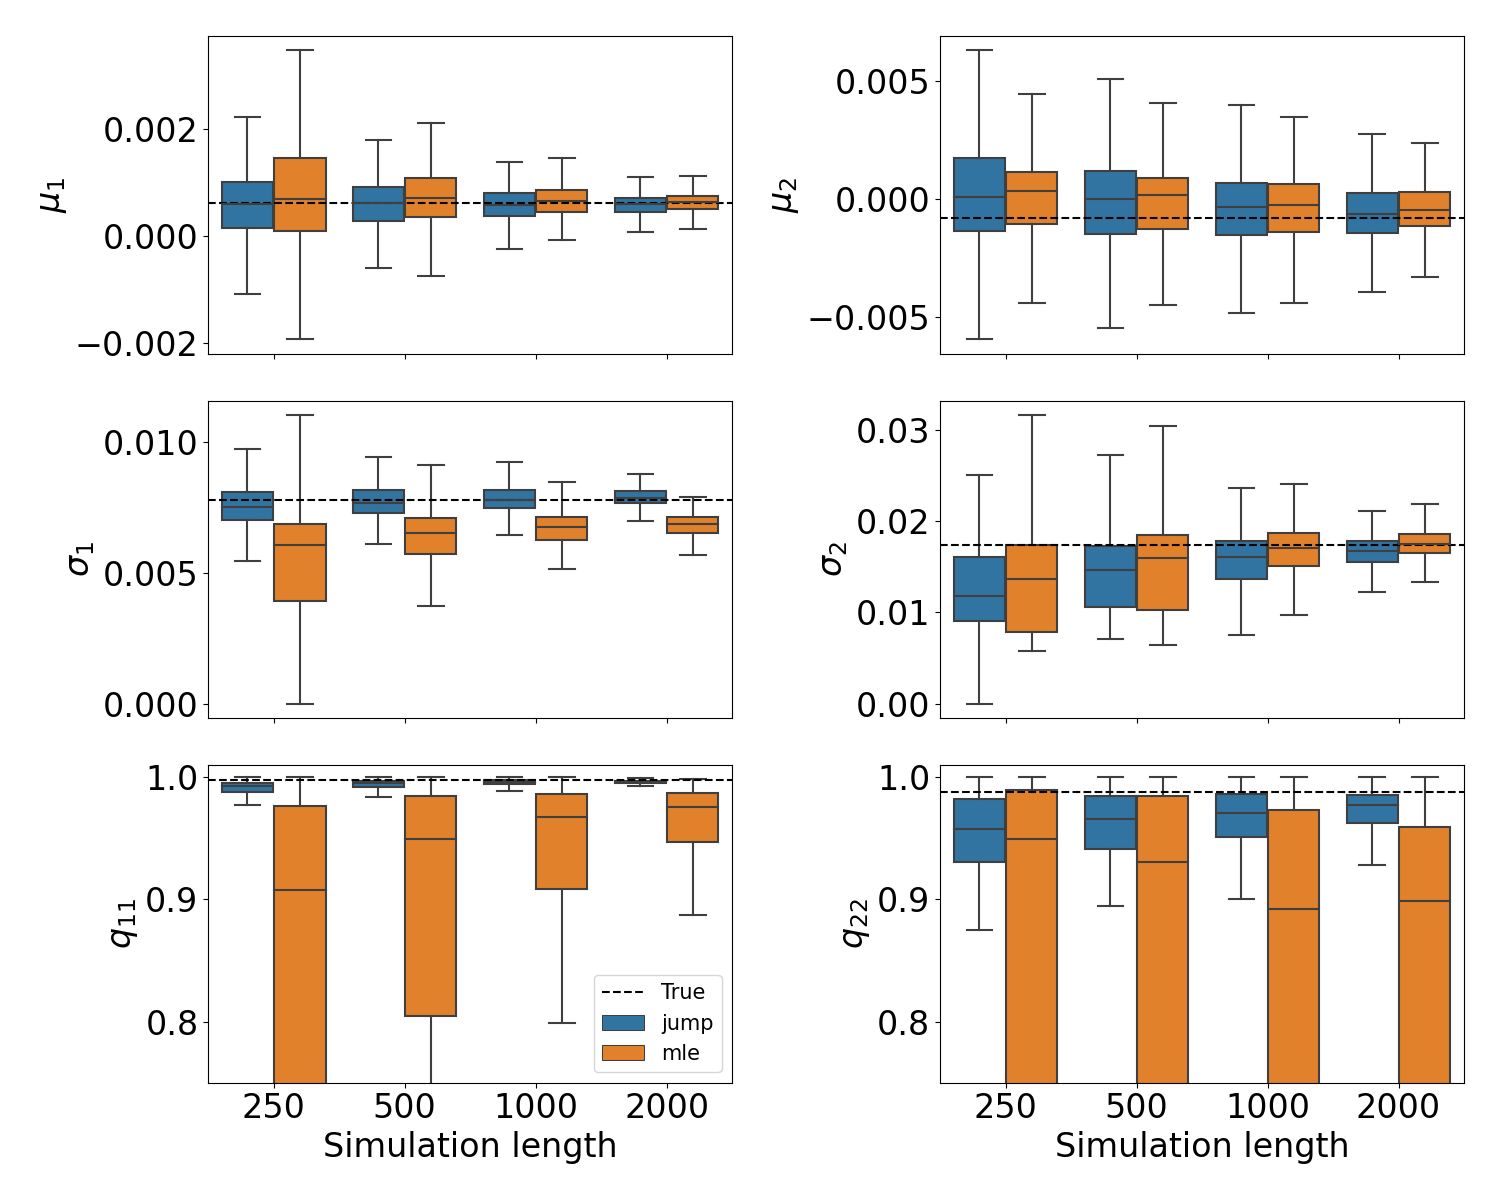
\includegraphics[width=1\textwidth]{analysis/model_convergence/images/simulation_t_box.png}
    
    \caption [Boxplot of \mle and \jump parameter estimates from miss-specified conditional t-distributions with five degrees of freedom] {Boxplot of the \mle and \jump parameter estimates from miss-specified t-distributions with five degrees of freedom. The estimates show the models' convergence towards the true parameter values as a function of simulation length. Results are based on 1000 simulations.}
    \label{fig:jump_t_box}
\end{figure}

This is in contrast to the \mle model, which assumes a given conditional distribution for each state during training. From \cref{fig:jump_t_box} it becomes clear that such an assumption has a sizeable error as the model generally doesn't perform well across the parameters. Most conspicuously, the \mle model has basically broken down in terms of the transition probabilities where it is very far from the true estimates, even at the largest sample sizes. This would result in states with very low persistence and frequent state switching. Here we note that the \mle model doesn't seem consistent for parameters $\sigma_1$, $q_{11}$ and $q_{22}$ as it is converging towards lower estimates than the true parameters, though variance is decreasing for all estimates. One could try to train the \mle model on larger sample sizes, to check its convergence of transition probabilities further, however, even if the model did eventually converge, given enough data, the problem is that financial returns are generally shown to have time varying features, (Ryden (1997), Nystrup et al. (2017)). As a result, one should be reluctant to consider estimating models on data that goes back too far, which is why the longest simulation length is 2000 observations. Just as before, \cref{fig:jump_t_box_2states} shows the same analysis but only using simulations where two states occur. As opposed to \cref{fig:jump_normal_box_2states} where the \mle model drastically improved, this is no longer the case when performed on t-distributed data. Though the \mle model does see slight improvement in $q_{11}$ it is still vastly misestimating $q_{22}$, and the variance even seem to increase with simulation length. Curiously, the \mle model is estimating conditional means and variance quite closely, so it will interesting to see its performance on real data. Future research should consider altering the \mle estimation to increase the values of transition probabilities, since these are essentially always underestimated. In a rolling model, one might constrain these probabilities to some threshold values to prevent them from crashing as they evidently do in \cref{fig:jump_t_box} or regularize how much they can change from one period to the next. In the next sections, we will impose $q_{11} \geq 0.90$ for the \mle estimator to ensure it does not crash in the low-variance state as it has done in this section. The choice of 0.90 is a trade-off between letting the HMM detect abrupt changes in cases of economic crashes, and constraining the model from letting persistence become too low, thereby sporadically jumping from state to state. As can be seen from the distribution of the \mle model's estimate of $q_{11}$ in \cref{fig:jump_t_box}, a transition probability of 0.90 is only barely part of the distribution for sample sizes of 1000 and 2000. As such this constraint is not expected to generally change the optimal parameters of the \mle moving forward, and only be active in 'outlier' cases. We note that no constraint is imposed on $q_{22}$, i.e. the high-variance state because this state is designed to catch fast increases in the variances of returns.

\begin{figure}[H] 
    \centering
    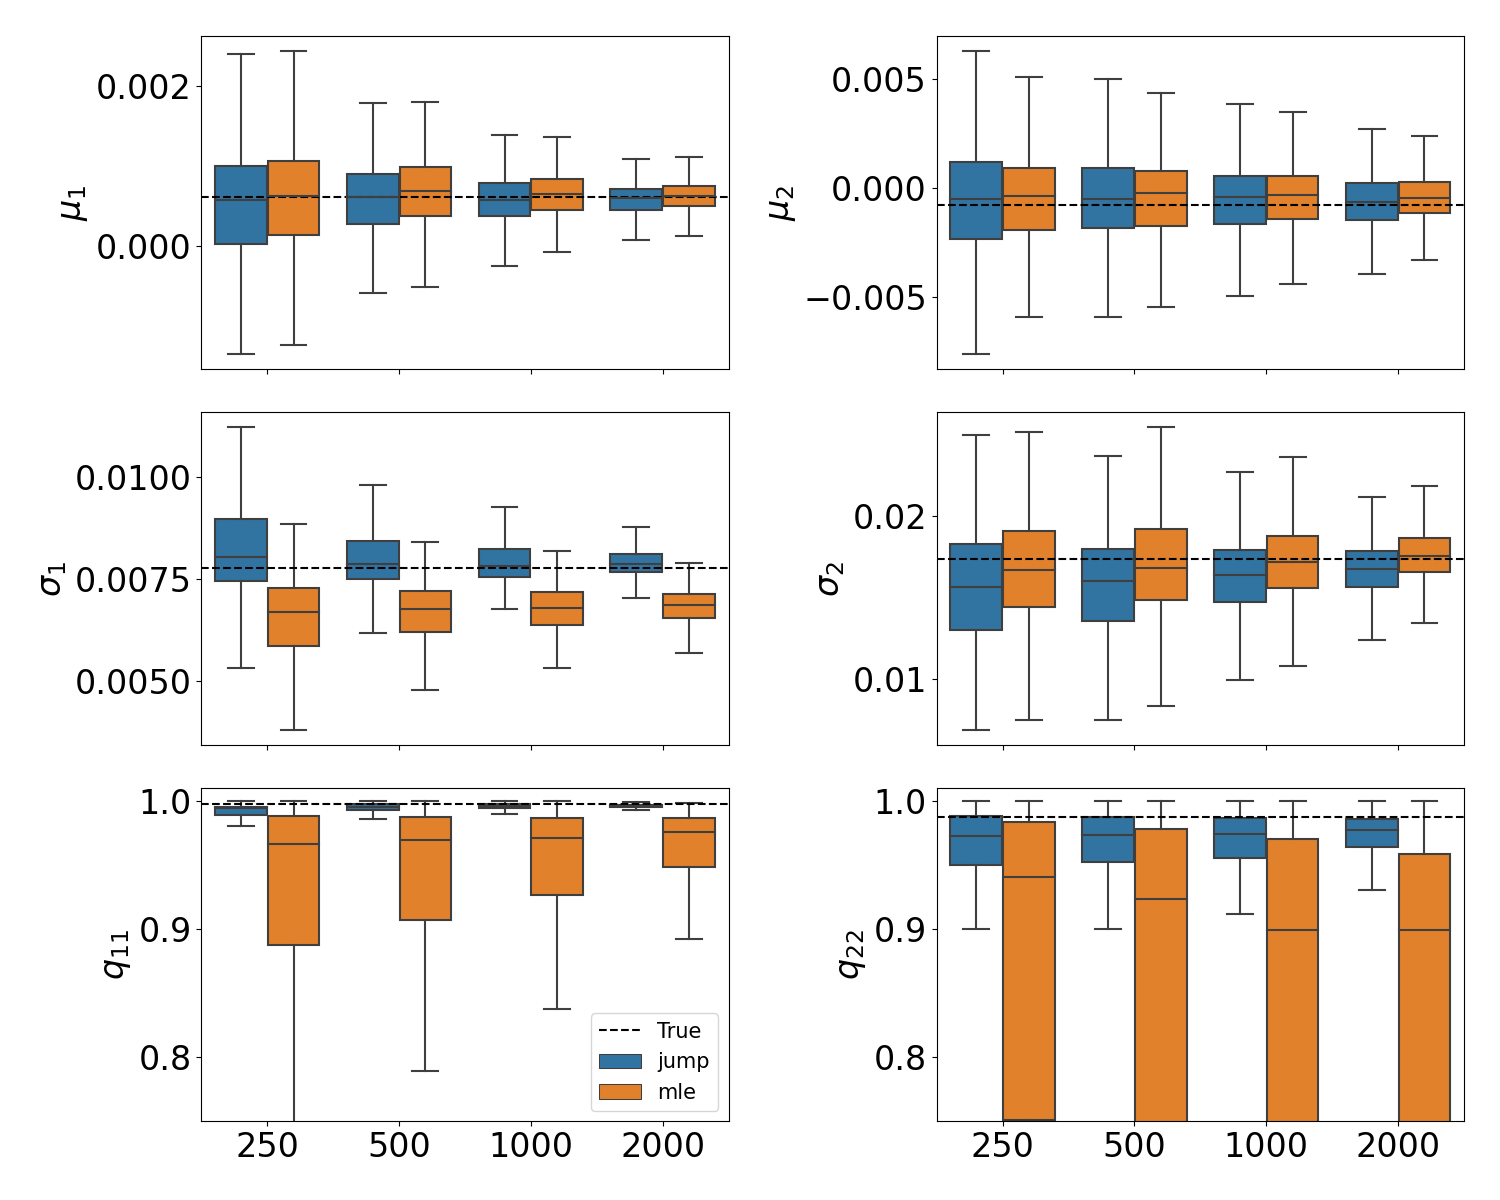
\includegraphics[width=1\textwidth]{analysis/model_convergence/images/simulation_t_box_2states.png}
    
    
    
    \caption[Boxplot of the \mle and \jump parameter estimates from miss-specified t-distributions with five degrees of freedom. Sorted version]{Boxplot of the \mle and \jump parameter estimates from miss-specified t-distributions with five degrees of freedom. The estimates show the models' convergence towards the true parameter values as a function of simulation length. Results are based on 1000 simulations which are sorted to only include those where both states are present}. \textbf{Consider moving to appendix.}
    \label{fig:jump_t_box_2states}
\end{figure}

In conclusion, testing the models' performance on data with misspecified distributions, has allowed us better understand how they might perform on real data, when the true values are unknown. The fact that the \jump model was shown to be very robust in terms of transition probabilities, is convincing of its merit on real data. As the \mle model generally had some problems with fitting the low-variance state, we have imposed $q_{11}\geq 0.90$ for the model in the remaining sections. As a final remark it should be noted that the results presented in this section is entirely based on data simulated from an HMM, thus with the underlying assumption that financial data to some degree can be explained by such a model. As a result, the next section will consist of an analysis of HMMs ability to reproduce stylized facts. This should provide further insight into their appropriateness as times series models.